\chapter{Exercise 04}
\extitle{Practicing Linear Regression}
\turnindir{ex04}
\exnumber{04}
\exfiles{linear\_model.py, are\_blue\_pills\_magics.csv}
\exforbidden{sklearn}
\makeheaderfilesforbidden


% ================================= %
\section*{Objective}
% --------------------------------- %
Evaluate a linear regression model on a very small dataset, with a given hypothesis function $h$.\
Manipulate the loss function $J$, plot it, and briefly analyze the plot.

% ================================= %
\section*{Instructions}
% --------------------------------- %
You can find in the \texttt{resources} folder a tiny dataset called \texttt{are\_blue\_pills\_magics.csv} which gives you the driving performance of space pilots as a function of the quantity of the "blue pills" they took before the test.
You have a description of the data in the file named \texttt{are\_blue\_pills\_magics.txt}.
As your hypothesis function $h$, you will choose:

$$
h_{\theta}(x) = \theta_0 + \theta_1x
$$

Where $x$ is the variable, and $\theta_0$ and $\theta_1$ are the coefficients of the hypothesis.
The hypothesis is a function of $x$.

\textbf{You are strongly encouraged to use the class you have implement in the previous exercise}.
\newline

Your program must:
\begin{itemize}
  \item Read the dataset from the csv file,
  \item perform a linear regression, 
\end{itemize}
\newpage
Then you will model the data and plot 2 different graphs:
\begin{itemize}
  \item A graph with the data and the hypothesis you get for the spacecraft piloting score versus the quantity of "blue pills" (see figure \ref{best fit for score vs micrograms})
  \begin{figure}[!h]
    \centering
    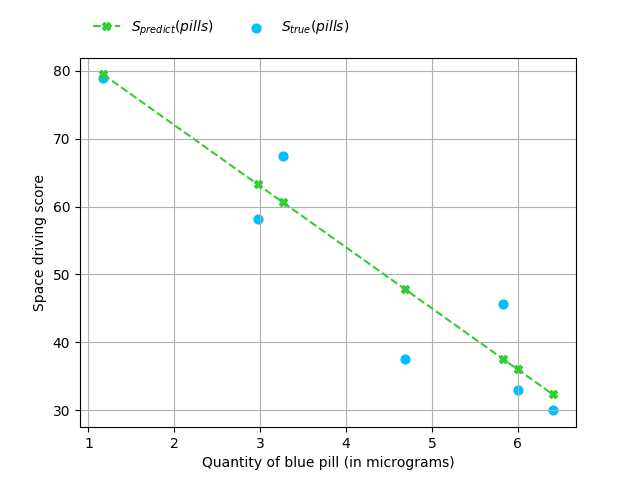
\includegraphics[scale=0.6]{assets/ex04_score_vs_bluepills.png}
    \caption{Space driving score as a function of the quantity of blue pill (in micrograms). In blue the real values and in green the predicted values.}
    \label{best fit for score vs micrograms}
  \end{figure}
  
  \item The loss function $J(\theta)$ in function of the $\theta$ values (see figure \ref{loss function qs function of theta1 and theta0}),
  \begin{figure}[!h]
    \centering
    \includegraphics[scale=0.6]{assets/ex04_J_vs_t1.png}
    \caption{Evolution of the loss function $J$ as a function of $\theta_1$ for different values of $\theta_0$.}
    \label{loss function qs function of theta1 and theta0}
  \end{figure}
   
  \item You will calculate the MSE of the hypothesis you chose (you know how to do it already).
\end{itemize}

% ================================= %
\section*{Examples}
% ================================= %
\begin{minted}[bgcolor=darcula-back,formatcom=\color{lightgrey},fontsize=\scriptsize]{python}
import pandas as pd
import numpy as np
from sklearn.metrics import mean_squared_error
from my_linear_regression import MyLinearRegression as MyLR

data = pd.read_csv("are_blue_pills_magic.csv")
Xpill = np.array(data['Micrograms']).reshape(-1,1)
Yscore = np.array(data['Score']).reshape(-1,1)

linear_model1 = MyLR(np.array([[89.0], [-8]]))
linear_model2 = MyLR(np.array([[89.0], [-6]]))
Y_model1 = linear_model1.predict_(Xpill)
Y_model2 = linear_model2.predict_(Xpill)

print(MyLR.mse_(Yscore, Y_model1))
# 57.60304285714282
print(mean_squared_error(Yscore, Y_model1))
# 57.603042857142825
print(MyLR.mse_(Yscore, Y_model2))
# 232.16344285714285
print(mean_squared_error(Yscore, Y_model2))
# 232.16344285714285
\end{minted}
\par
Here, the use of scikit learn is to ensure that our code is performing as expected. The use of scikit learn is forbidden in the code you will turn-in.

\hint{
There is no method named \texttt{.mse\_} in sklearn's LinearRegression class, but there is also a method named \texttt{.score}.
The \texttt{.score} method corresponds to the $R^2$ score.
The metric MSE is available in the \texttt{sklearn.metrics} module.
}